\begin{refsection}
  \begin{frame}{Checkpoint Released Timeline and Model Architectures}
    \begin{columns}[T,onlytextwidth]
      \begin{column}{0.65\textwidth}
        % \vspace{0.3em}
        \begin{itemize}[leftmargin=0.2em]
            \item \textcolor{violet}{【Stability AI】} \textcolor{gray}{Stable Diffusion 2.1: 2022/12/06}
            \item \textcolor{teal}{【Meta AI】} \textcolor{black}{DiT: 2023/01/08}
            \item \textcolor{violet}{【Stability AI】} \textcolor{gray}{Stable Diffusion XL 1.0: 2023/07/26}
            \item \textcolor{red}{【Huawei】} \textcolor{black}{PixArt-\alpha: 2023/10/06}
            \item \textcolor{red}{【Huawei】} \textcolor{black}{PixArt-\delta: 2024/01/10}
            \item \textcolor{cyan}{【Shanghai AI Lab】} \textcolor{black}{Lumina-T2I: 2024/04/01}
            \item \textcolor{red}{【Huawei】} \textcolor{black}{PixArt-Σ: 2024/04/11}
            \item \textcolor{cyan}{【Shanghai AI Lab】} \textcolor{black}{Lumina-Next-T2I: 2024/05/12}
            \item \textcolor{violet}{【Stability AI】} \textcolor{black}{Stable Diffusion 3: 2024/06/12}
            \item \textcolor{black}{【Black Forest Lab】} \textcolor{black}{Flux.1}
            \item \textcolor{violet}{【Stability AI】} \textcolor{black}{Stable Diffusion 3.5: 2024/10/22}
            \item \textcolor{green!70!black}{【NVIDIA】} \textcolor{black}{SANA: 2025/01/11}
            \item \textcolor{cyan}{【Shanghai AI Lab】} \textcolor{black}{Lumina-Image-2.0: 2025/01/22}
            \item \textcolor{green!70!black}{【NVIDIA】} \textcolor{black}{SANA 1.5: 2025/03/21}
        \end{itemize}
      \end{column}
      \begin{column}{0.35\textwidth}
        \centering
        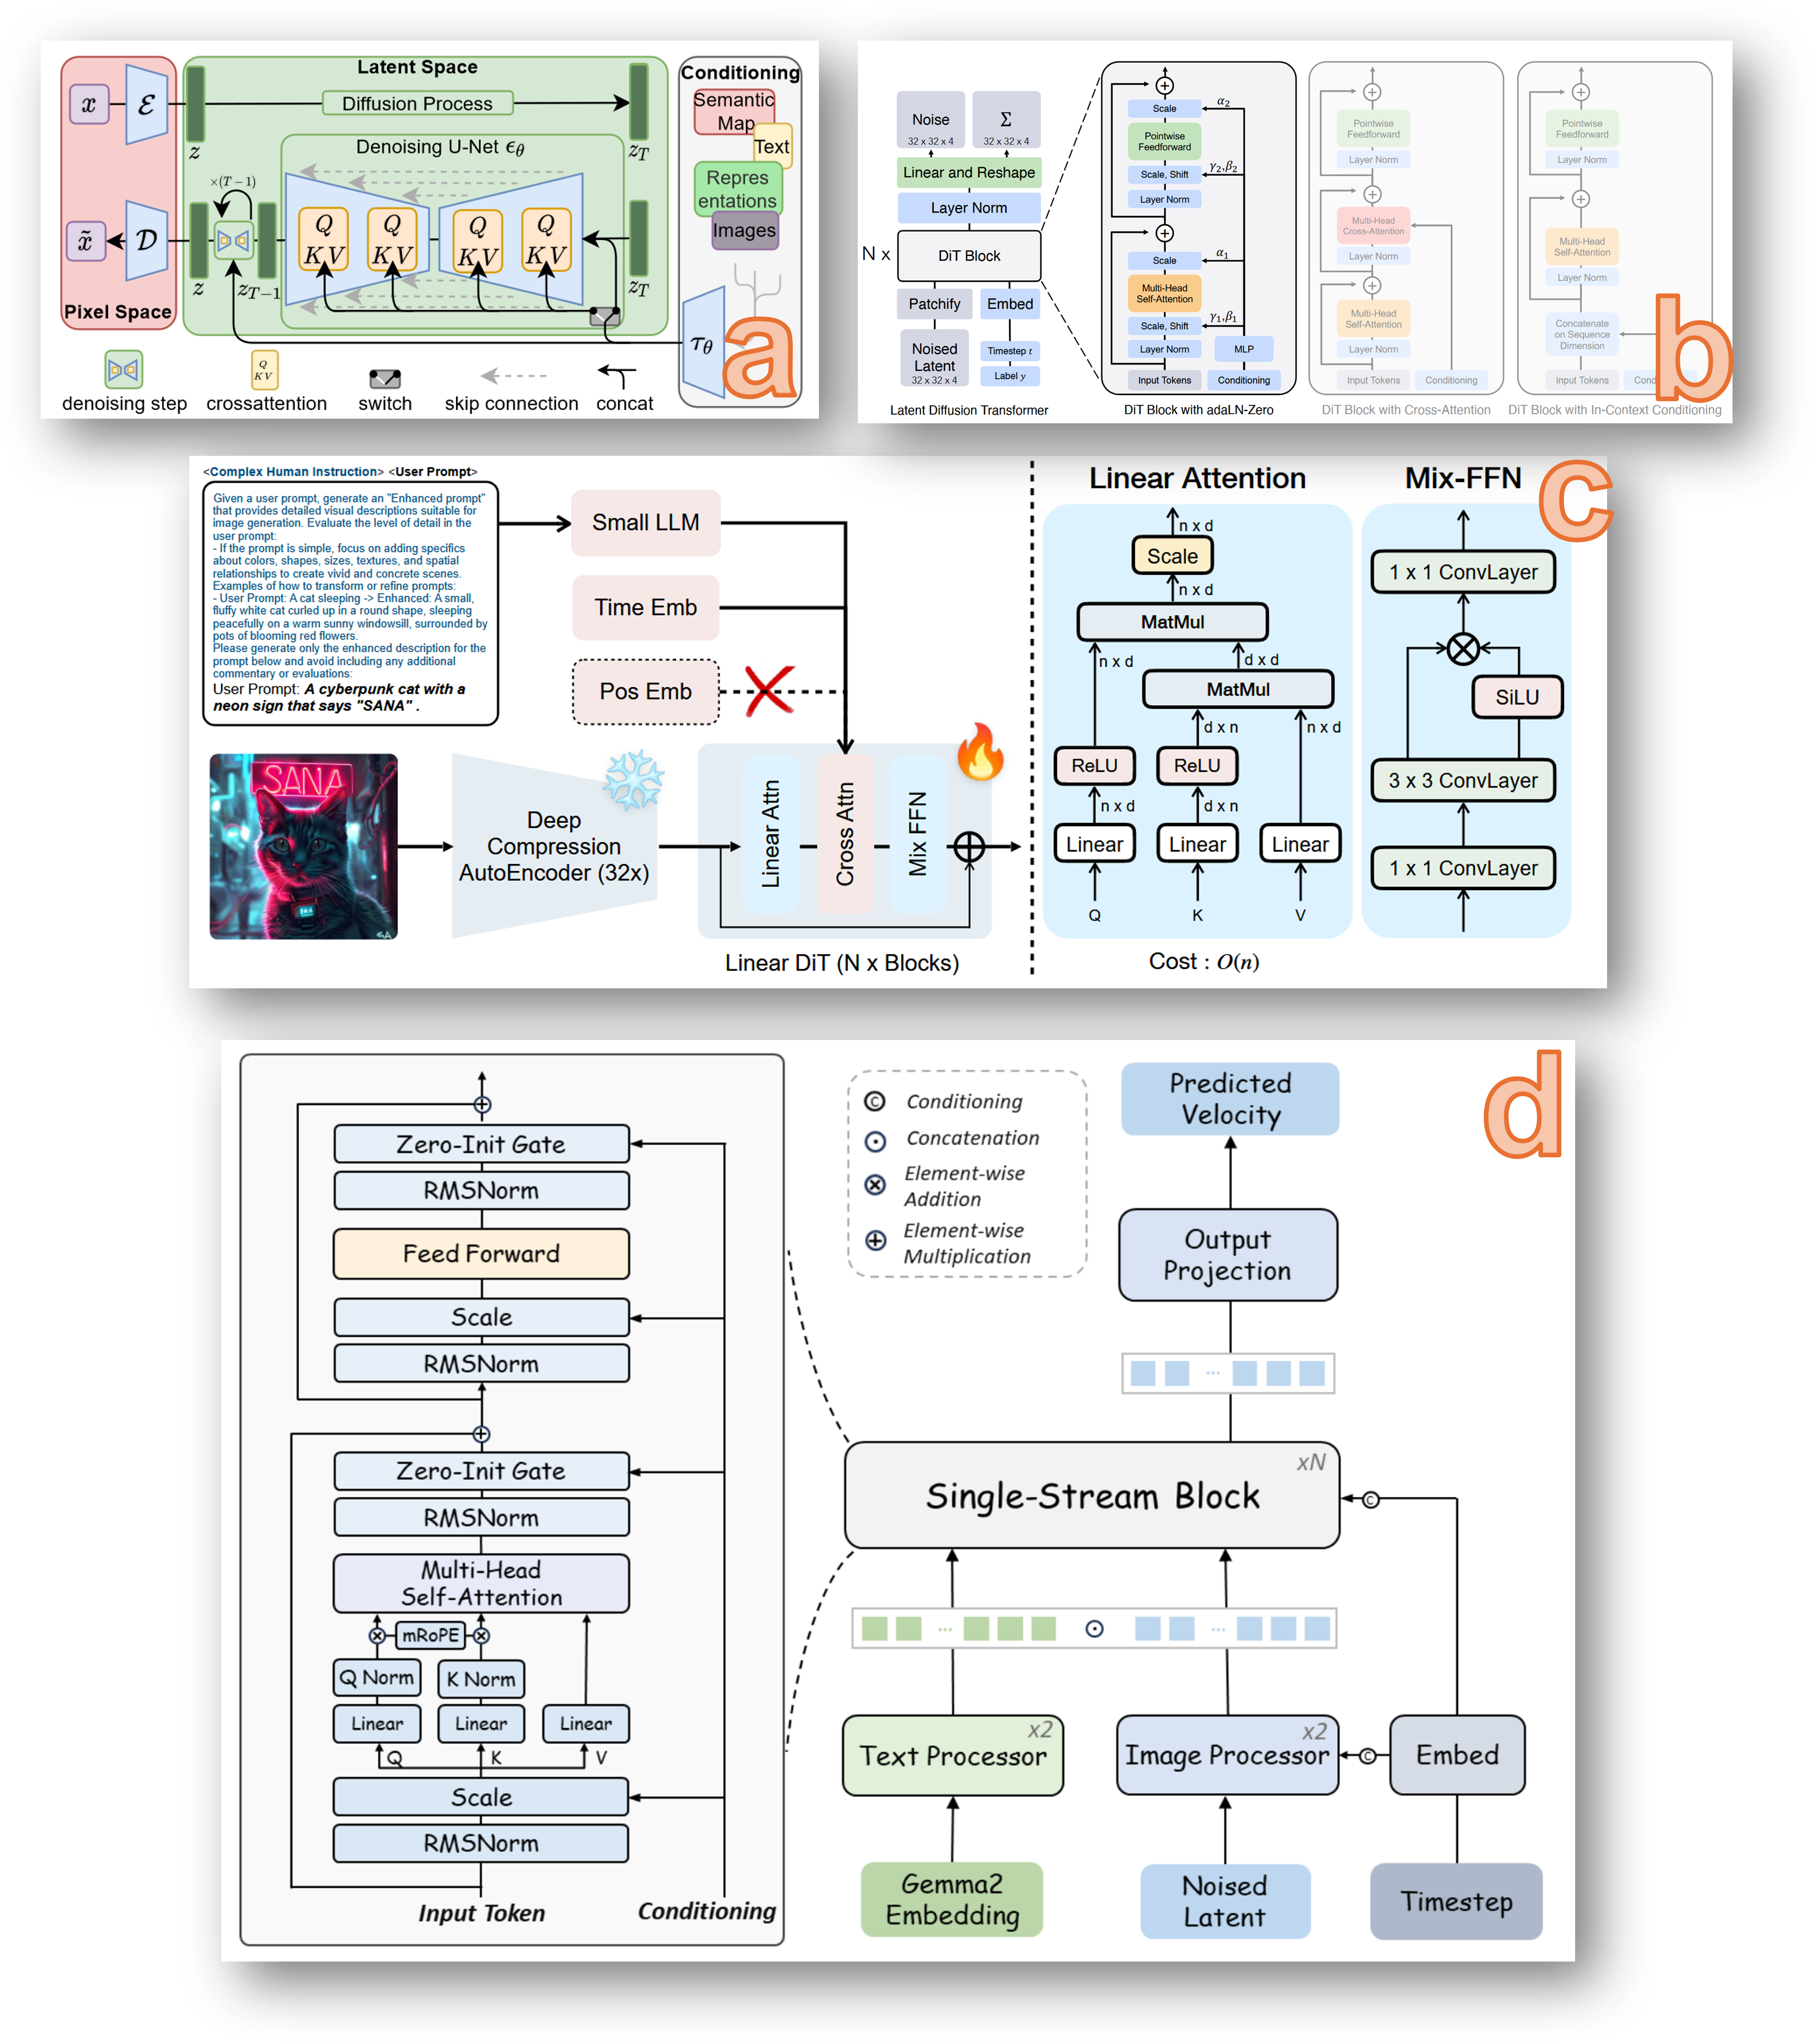
\includegraphics[width=\linewidth]{figure1.png}
        \vspace{0.4em}

        {\scriptsize
        a. Unet b. DiTs \\ 
        c. Linear DiTs d. Next-DiTs
        }
      \end{column}
    \end{columns}
    \bottomleftrefs
  \end{frame}
\end{refsection}

\begin{refsection}
\begin{frame}{Diffusion Transformer (DiT)}

  \centering
  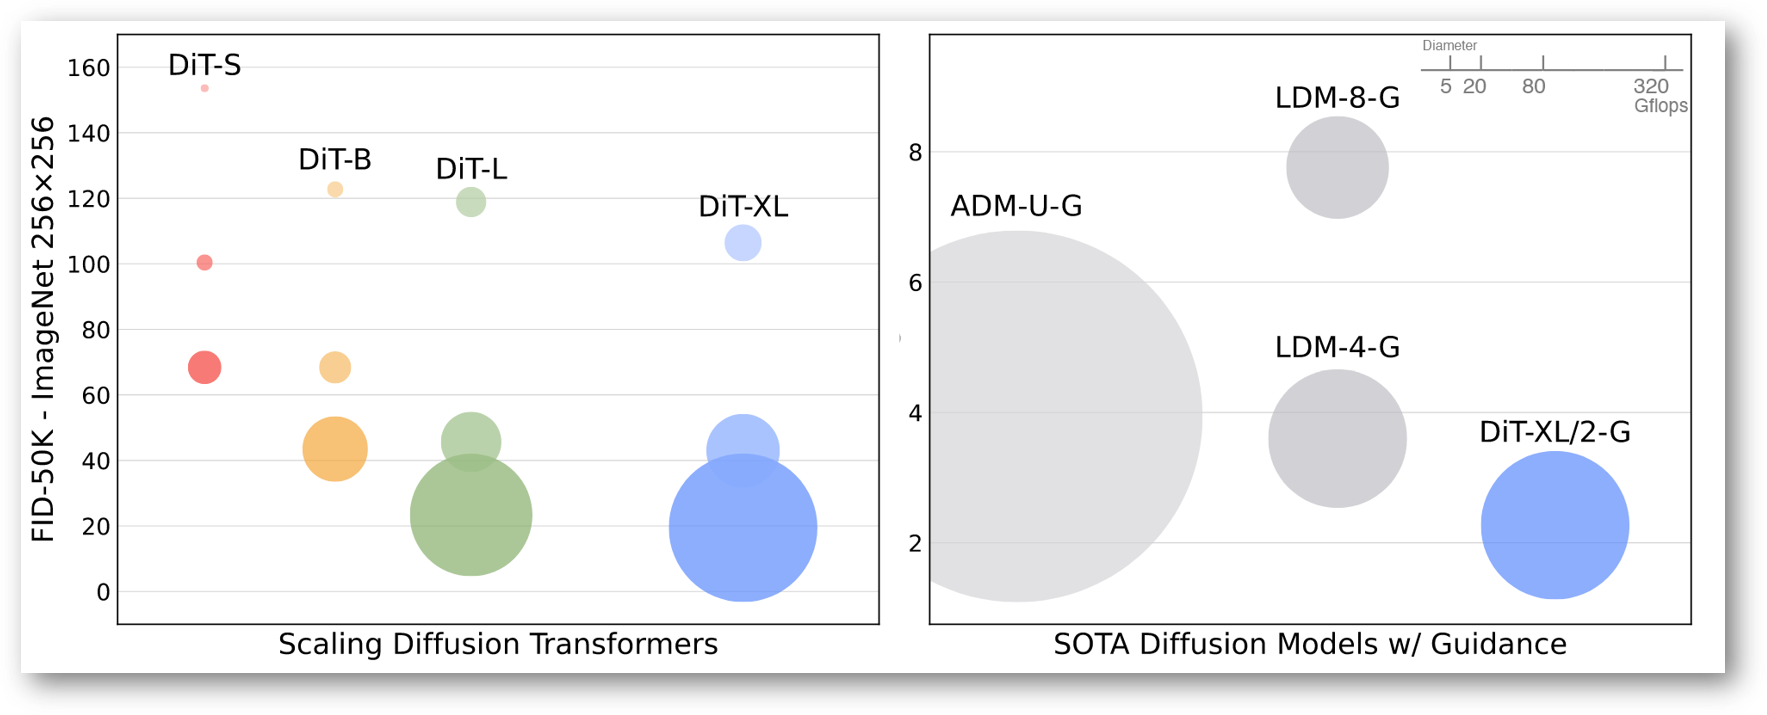
\includegraphics[width=0.87\linewidth]{figure2.png}
  
  \vspace{0.7em}
  {\scriptsize
    \textbf{ImageNet generation with Diffusion Transformers (DiTs)~\parencite{Peebles_2023_ICCV}.} Bubble area indicates the FLOPs of the diffusion model.
    \textbf{Left:} FID-50K (lower is better) of DiT models at 400K training iterations, showing improved performance with increased FLOPs.
    \textbf{Right:} DiT-XL/2 is compute-efficient and outperforms all prior U-Net-based diffusion models (e.g., ADM, LDM).
  }


\bottomleftrefs
\end{frame}
\end{refsection}

\begin{refsection}
  \begin{frame}{Diffusion Transformer (DiT)}
  
    \centering
    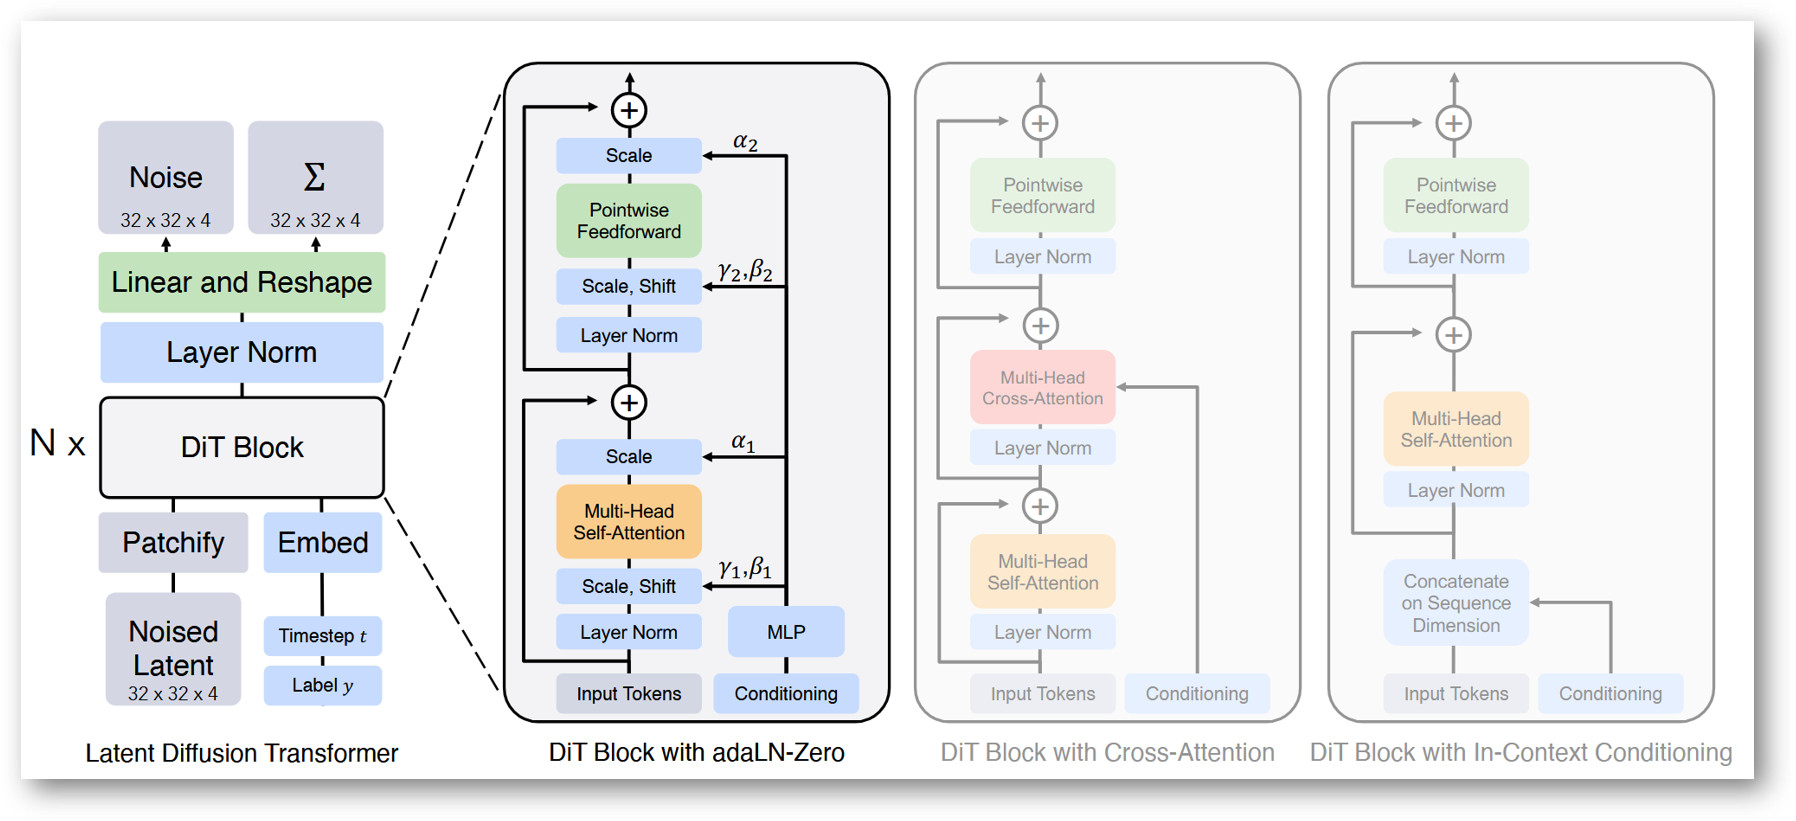
\includegraphics[width=0.87\linewidth]{figure3.png}
    
    % \vspace{0.7em}
    {\scriptsize
    The Diffusion Transformer (DiT)~\parencite{Peebles_2023_ICCV} architecture. Left: We train conditional latent DiT models. The input latent is decomposed into patches and processed by several DiT blocks. Right: Details of our DiT blocks. We experiment with variants of standard transformer blocks that incorporate conditioning via adaptive layer norm, cross-attention and extra input tokens. Adaptive layer norm works best.
    }
  
  
  \bottomleftrefs
  \end{frame}
  \end{refsection}

  \begin{refsection}
    \begin{frame}{Diffusion Transformer (DiT)}
    
      \centering
      \includegraphics[width=0.87\linewidth]{figure4.png}
      
      % \vspace{0.7em}
      {\scriptsize
      Input specifications for DiT~\parencite{Peebles_2023_ICCV}. Given a patch size \( p \times p \), a spatial representation (the noised latent from the VAE) of shape \( I \times I \times C \) is "patchified" into a sequence of length \( T = (I/p)^2 \) with hidden dimension \( d \). A smaller patch size \( p \) results in a longer sequence and thus more GFLOPs.
      }
    
    \bottomleftrefs
    \end{frame}
    \end{refsection}
  

\begin{refsection}
  \begin{frame}{PixArt-\alpha}
    \centering
    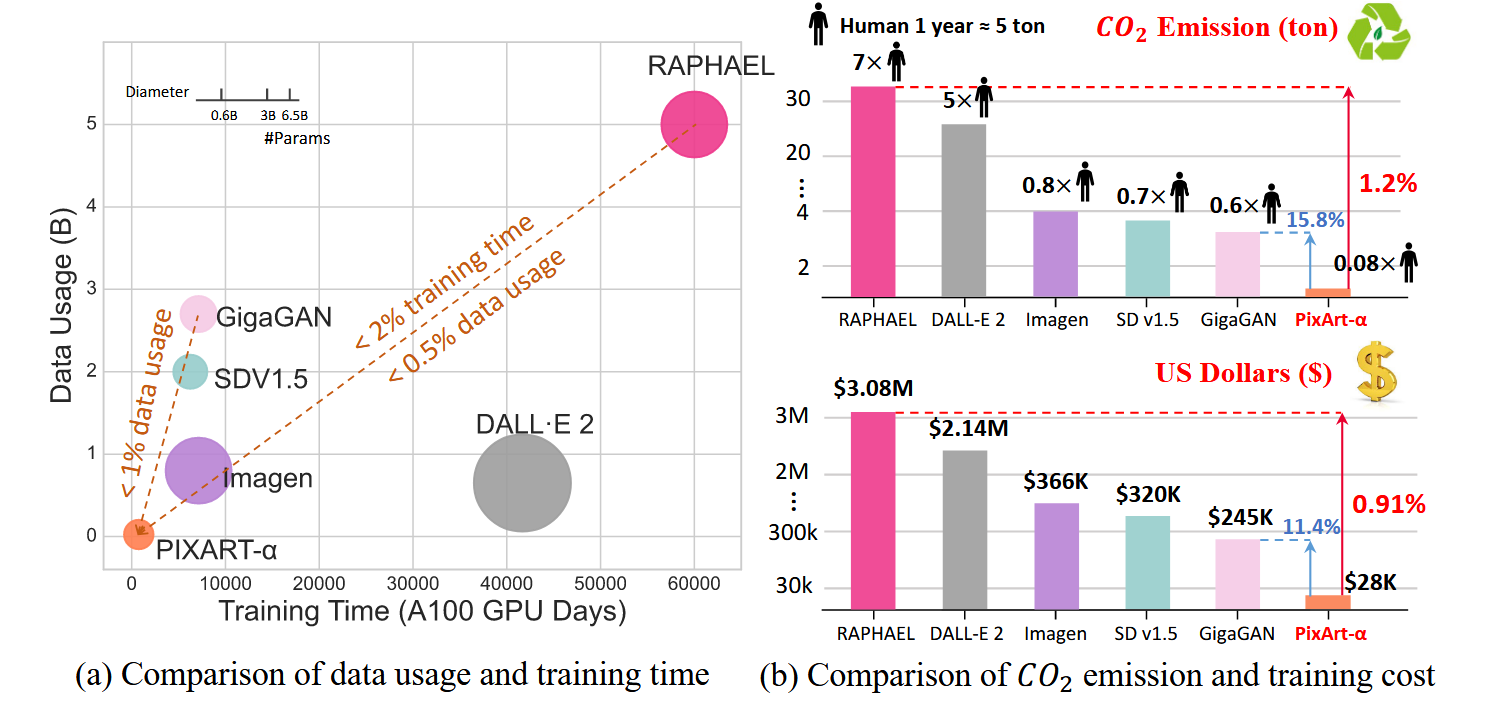
\includegraphics[width=0.87\linewidth]{figure5.png}

    {\scriptsize
    Comparisons of CO$_2$ emissions and training cost among T2I generators. PixART-$\alpha$~\parencite{chenPixArtaFastTraining2023} achieves an exceptionally low training cost of \$28,400. Compared to RAPHAEL, our CO$_2$ emissions and training costs are merely 1.2\% and 0.91\%, respectively.
    }
    \bottomleftrefs
  \end{frame}
\end{refsection}

\begin{refsection}
  \begin{frame}{PixArt-\alpha~\&~PixArt-\delta}
    \centering
    \begin{minipage}{0.3\linewidth}
      \centering
      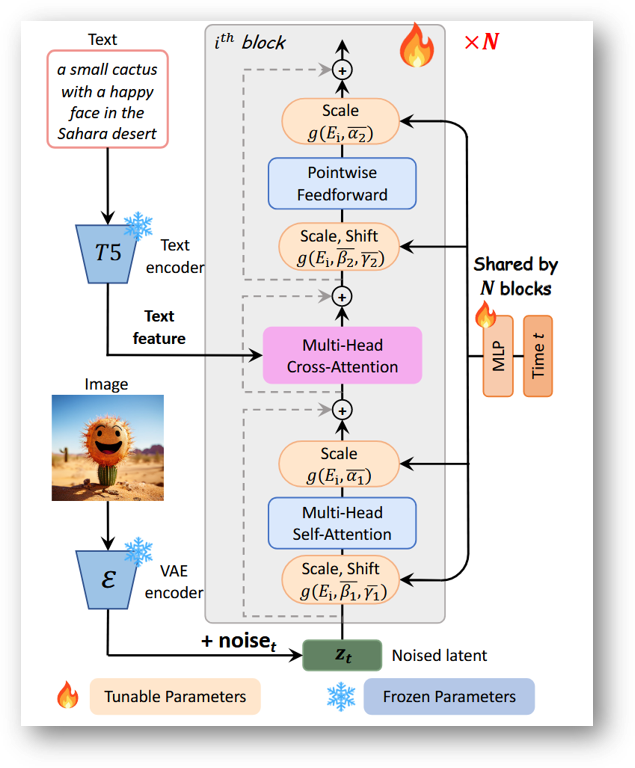
\includegraphics[width=\linewidth]{figure6a.png}
    \end{minipage}
    \hfill
    \begin{minipage}{0.35\linewidth}
      \centering
      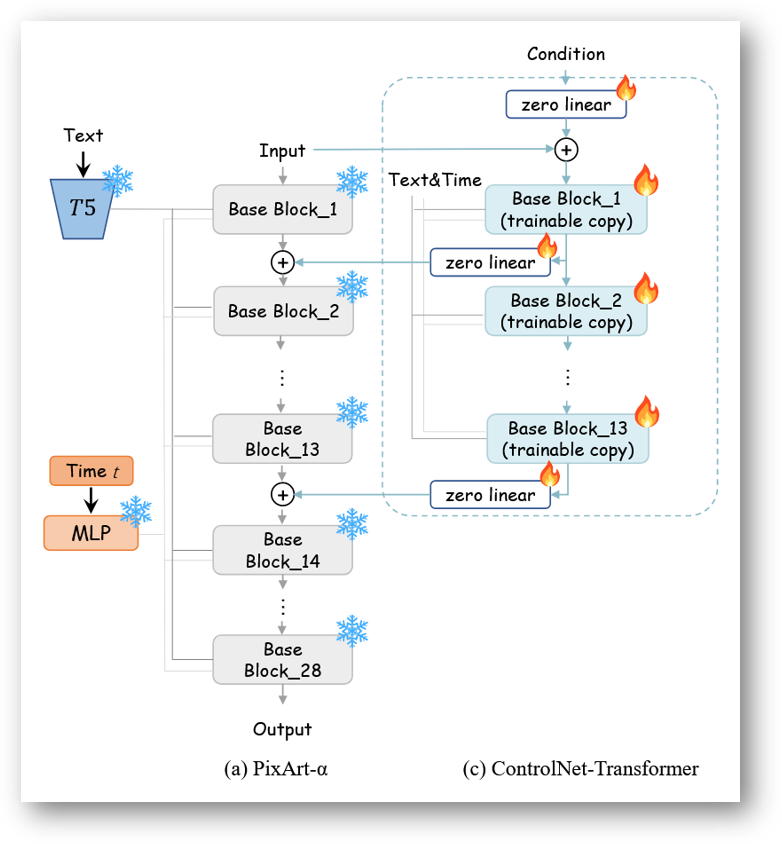
\includegraphics[width=\linewidth]{figure6b.png}
    \end{minipage}

    {\scriptsize
    Left: Model architecture of PixArt-\alpha~\parencite{chenPixArtaFastTraining2023}. To optimize efficiency, all blocks share the same adaLN-single parameters for time conditions. Right: PixArt-\delta~\parencite{chenPIXARTdFastControllable2024} integrated with ControlNetTransformer.      
    }
    \bottomleftrefs
  \end{frame}
\end{refsection}

\begin{refsection}
  \begin{frame}{Stable Diffusion 3}
    \centering
    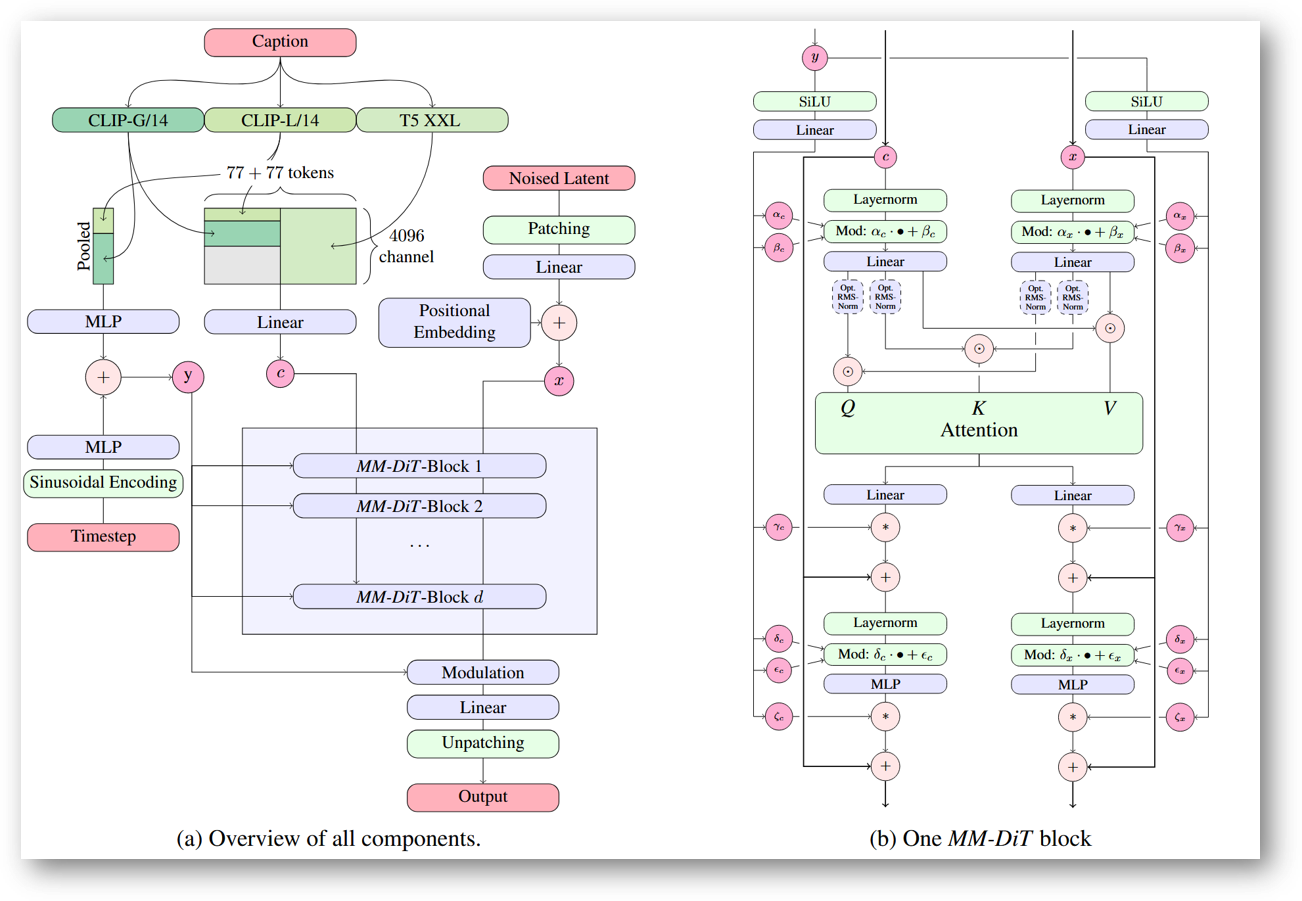
\includegraphics[width=0.65\linewidth]{figure7.png}

    {\scriptsize
    SD3~\parencite{esserScalingRectifiedFlow2024a} model architecture. Concatenation is indicated by $\odot$, and element-wise multiplication by $*$. RMS-Norm for Q and K can be added to stabilize training runs.
    }
    \bottomleftrefs
  \end{frame}
\end{refsection}

\begin{refsection}
  \begin{frame}{SANA}
    \centering
    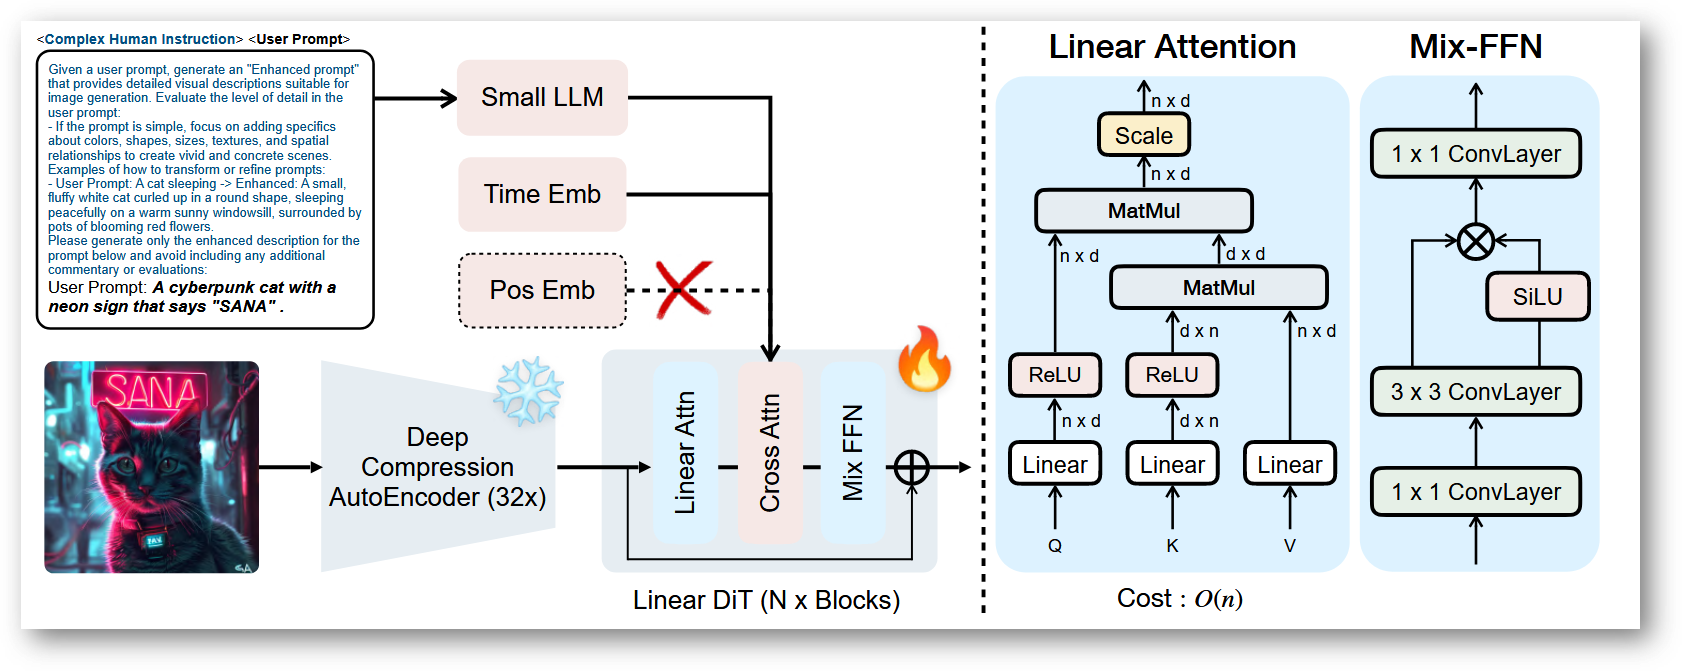
\includegraphics[width=0.87\linewidth]{figure8.png}

    {\scriptsize
    Overview of Sana~\parencite{xieSANAEfficientHighResolution2024}: Fig. (a) describes the high-level training pipeline, containing our 32× deep compression Autoencoder, Linear DiT, and complex human instruction. Note that Positional embedding is not required in our framework. Fig. (b) describes the detailed design of the Linear Attention and Mix-FFN in Linear DiTs.
    }
    \bottomleftrefs
  \end{frame}
\end{refsection}

\begin{refsection}
  \begin{frame}{Lumina-Image 2.0
    }
    \centering
    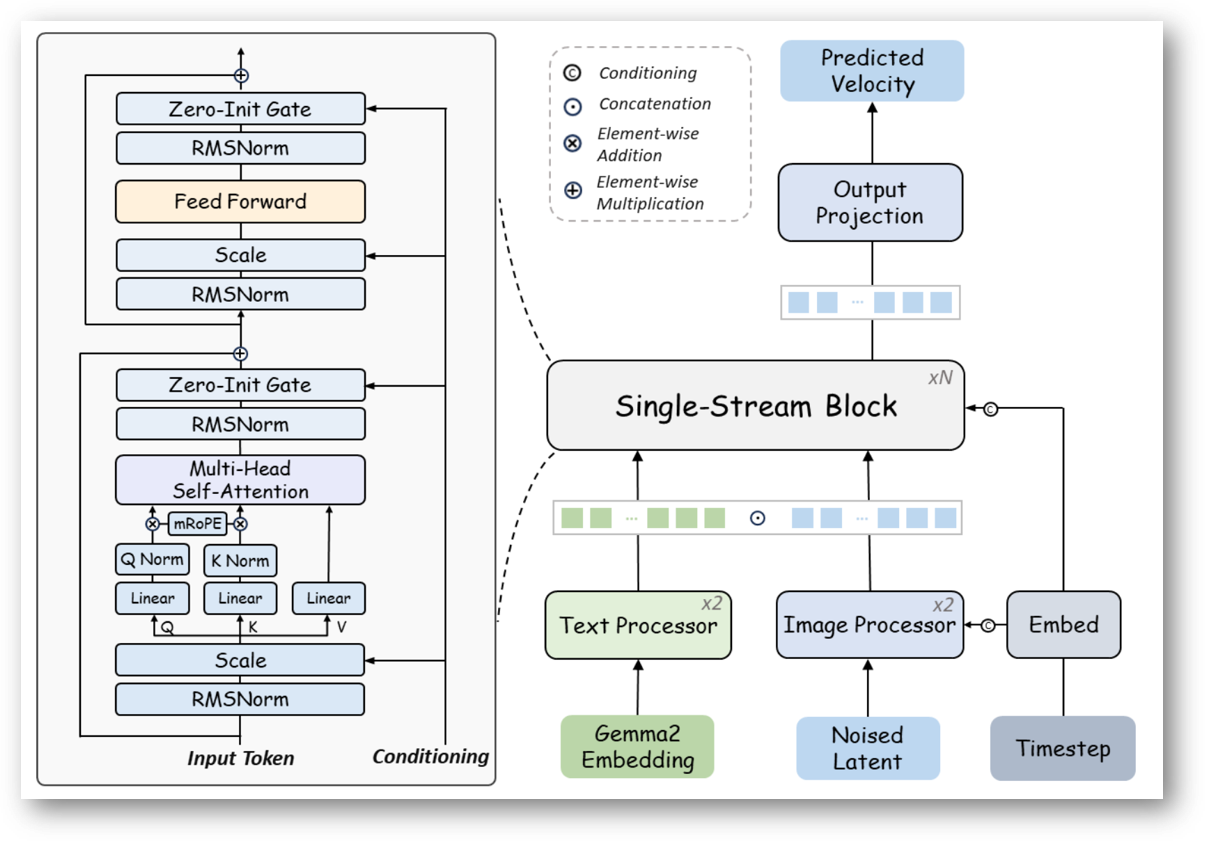
\includegraphics[width=0.6\linewidth]{figure9.png}

    {\scriptsize
    Overview of Lumina-Image 2.0~\parencite{qinLuminaImage20Unified2025}.
    }
    \bottomleftrefs
  \end{frame}
\end{refsection}